% -----------------------------------------------
% Template for ISMIR Papers
% 2016 version, based on previous ISMIR templates

% Requirements :
% * 6+1 page length maximum
% * 2MB maximum file size
% * Copyright note must appear in the bottom left corner of first page
% (see conference website for additional details)
% -----------------------------------------------

\documentclass{article}
\usepackage{ismir,amsmath,cite}
\usepackage{graphicx}
\usepackage{color}

% Title.
% ------
\title{Topological Beat Tracking with Laplacian Circular Coordinates}

% Note: Please do NOT use \thanks or a \footnote in any of the author markup

% Single address
% To use with only one author or several with the same address
% ---------------
%\oneauthor
% {Names should be omitted for double-blind reviewing}
% {Affiliations should be omitted for double-blind reviewing}

% Two addresses
% --------------
%\twoauthors
%  {First author} {School \\ Department}
%  {Second author} {Company \\ Address}

%% To make customize author list in Creative Common license, uncomment and customize the next line
%  \def\authorname{First Author, Second Author} 


% Three addresses
% --------------
\oneauthor
  {Christopher J. Tralie} {Duke University Department of Electrical And Computer Engineering \\ {\tt chris.tralie@gmail.com}}

%% To make customize author list in Creative Common license, uncomment and customize the next line
%  \def\authorname{First Author, Second Author, Third Author} 

% Four or more addresses
% OR alternative format for large number of co-authors
% ------------
%\multauthor
%{First author$^1$ \hspace{1cm} Second author$^1$ \hspace{1cm} Third author$^2$} { \bfseries{Fourth author$^3$ \hspace{1cm} Fifth author$^2$ \hspace{1cm} Sixth author$^1$}\\
%  $^1$ Department of Computer Science, University , Country\\
%$^2$ International Laboratories, City, Country\\
%$^3$  Company, Address\\
%{\tt\small CorrespondenceAuthor@ismir.edu, PossibleOtherAuthor@ismir.edu}
%}
%\def\authorname{First author, Second author, Third author, Fourth author, Fifth author, Sixth author}


\sloppy % please retain sloppy command for improved formatting

\begin{document}

%
\maketitle
%
\begin{abstract}
The abstract should be placed at the top left column and should contain about 150-200 words.
\end{abstract}
%
\section{Introduction}\label{sec:introduction}


%\begin{table}
% \begin{center}
% \begin{tabular}{|l|l|}
%  \hline
%  String value & Numeric value \\
%  \hline
%  Hello ISMIR  & \conferenceyear \\
%  \hline
% \end{tabular}
%\end{center}
% \caption{Table captions should be placed below the table.}
% \label{tab:example}
%\end{table}

%\begin{figure}
% \centerline{\framebox{
% 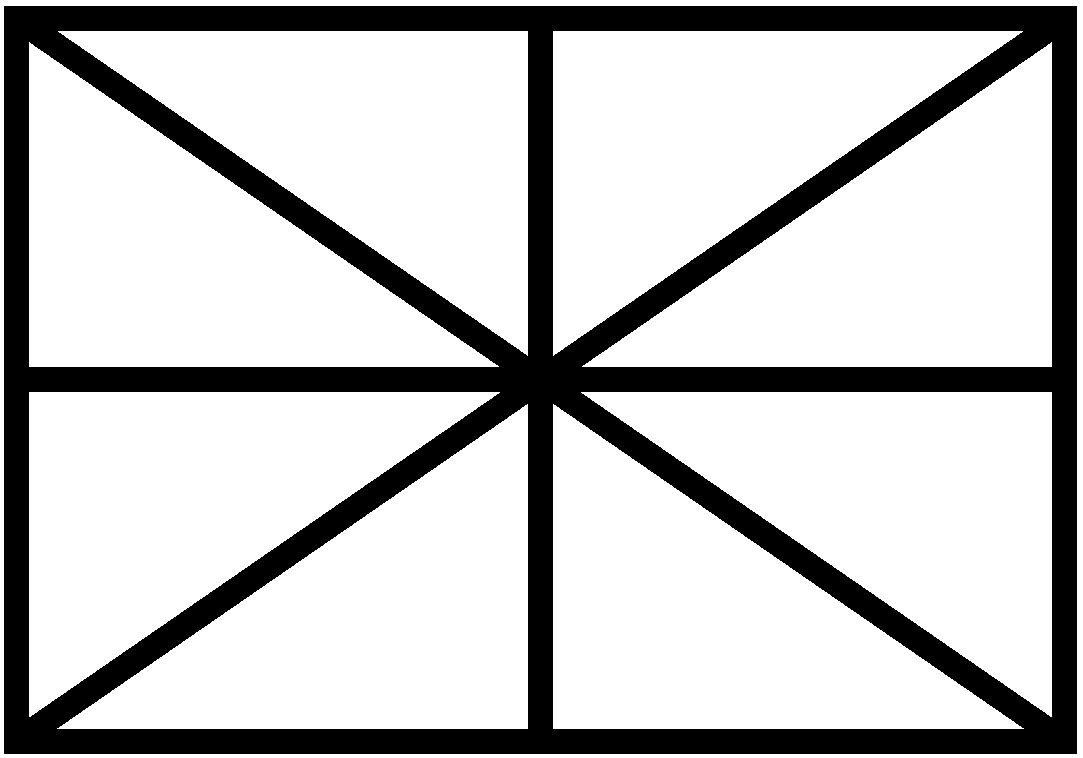
\includegraphics[width=\columnwidth]{figure.png}}}
% \caption{Figure captions should be placed below the figure.}
% \label{fig:example}
%\end{figure}



% For bibtex users:
\bibliography{LaplacianBeatTracking}


\end{document}
